%%%%%%%%%%%%%%%%%%%%%%%%%%%%%%%%%%%%%%%%%%%%%%%%%%%%%%%%%%%%%%%%%%%%
%% I, the copyright holder of this work, release this work into the
%% public domain. This applies worldwide. In some countries this may
%% not be legally possible; if so: I grant anyone the right to use
%% this work for any purpose, without any conditions, unless such
%% conditions are required by law.
%%%%%%%%%%%%%%%%%%%%%%%%%%%%%%%%%%%%%%%%%%%%%%%%%%%%%%%%%%%%%%%%%%%%

\documentclass[
  digital,     %% The `digital` option enables the default options for the
               %% digital version of a document. Replace with `printed`
               %% to enable the default options for the printed version
               %% of a document.
%%  color,       %% Uncomment these lines (by removing the %% at the
%%               %% beginning) to use color in the printed version of your
%%               %% document
  oneside,     %% The `oneside` option enables one-sided typesetting,
               %% which is preferred if you are only going to submit a
               %% digital version of your thesis. Replace with `twoside`
               %% for double-sided typesetting if you are planning to
               %% also print your thesis. For double-sided typesetting,
               %% use at least 120 g/m² paper to prevent show-through.
  nosansbold,  %% The `nosansbold` option prevents the use of the
               %% sans-serif type face for bold text. Replace with
               %% `sansbold` to use sans-serif type face for bold text.
  nocolorbold, %% The `nocolorbold` option disables the usage of the
               %% blue color for bold text, instead using black. Replace
               %% with `colorbold` to use blue for bold text.
  lof,         %% The `lof` option prints the List of Figures. Replace
               %% with `nolof` to hide the List of Figures.
  lot,         %% The `lot` option prints the List of Tables. Replace
               %% with `nolot` to hide the List of Tables.
]{fithesis4}
%% The following section sets up the locales used in the thesis.
\usepackage[resetfonts]{cmap} %% We need to load the T2A font encoding
\usepackage[T1,T2A]{fontenc}  %% to use the Cyrillic fonts with Russian texts.
\usepackage[
  main=english, %% By using `czech` or `slovak` as the main locale
                %% instead of `english`, you can typeset the thesis
                %% in either Czech or Slovak, respectively.
  english, german, russian, czech, slovak %% The additional keys allow
]{babel}        %% foreign texts to be typeset as follows:
%%
%%   \begin{otherlanguage}{german}  ... \end{otherlanguage}
%%   \begin{otherlanguage}{russian} ... \end{otherlanguage}
%%   \begin{otherlanguage}{czech}   ... \end{otherlanguage}
%%   \begin{otherlanguage}{slovak}  ... \end{otherlanguage}
%%
%% For non-Latin scripts, it may be necessary to load additional
%% fonts:
\usepackage{paratype}
\def\textrussian#1{{\usefont{T2A}{PTSerif-TLF}{m}{rm}#1}}
%%
%% The following section sets up the metadata of the thesis.
\thesissetup{
    date        = \the\year/\the\month/\the\day,
    university  = mu,
    faculty     = fi,
    type        = bc,
    department  = Department of Computer Systems and Communications,
    author      = Tomáš Zobač,
    gender      = m,
    advisor     = {RNDr. Rudolf Wittner},
    title       = {Implementation of provenance chains traversal},
    TeXtitle    = {Implementation of provenance chains traversal},
    keywords    = {Java, provenance, SOBHA, ÚVT, W3C PROV, PROV-DM},
    TeXkeywords = {Java, provenance, SOBHA, ÚVT, W3C PROV, PROV-DM},
    abstract    = {%
      Provenance is information documenting the history of an object. It can hold information, such as the origin of an object or previous actions performed on it. This information can be serialized into one of the many supported representations (e.g., PROV-N, XML) and subsequently interconnected, creating a provenance chain. This thesis aims to implement a tool for traversing provenance chains represented by PROV-N files, retrieving information about the precursors or successors of an entity represented in one of the files in the current chain, and optionally retrieving the type of actions performed on the documented object. The implementation will simulate the operational environment by providing a command-line user interface from where the user can call the mentioned actions on a set of pre-generated provenance files. In addition to the traversing operations, it will also implement the generation of provenance metadata to make the simulation of a traversal possible.
    },
    thanks      = {%
        I want to express my sincere gratitude to my thesis advisor, RNDr. Rudolf Wittner, for the valuable and extensive feedback and support he provided throughout the writing and implementation of my thesis.

        My family, and especially my girlfriend, were an immense source of support during my studies and while working on my thesis. Their constant encouragement was invaluable, and I am deeply grateful for it.
    },
    bib         = citations.bib,
    %% Remove the following line to use the JVS 2018 faculty logo.
    facultyLogo = fithesis-fi,
}
\usepackage{makeidx}      %% The `makeidx` package contains
\makeindex                %% helper commands for index typesetting.
%% These additional packages are used within the document:
\usepackage{paralist} %% Compact list environments
\usepackage{amsmath}  %% Mathematics
\usepackage{amsthm}
\usepackage{amsfonts}
\usepackage{url}      %% Hyperlinks
\usepackage{markdown} %% Lightweight markup
\usepackage{listings} %% Source code highlighting
\usepackage{dirtree}
\usepackage{fancyvrb}
\lstset{
  basicstyle      = \ttfamily,
  identifierstyle = \color{black},
  keywordstyle    = \color{blue},
  keywordstyle    = {[2]\color{cyan}},
  keywordstyle    = {[3]\color{olive}},
  stringstyle     = \color{teal},
  commentstyle    = \itshape\color{magenta},
  breaklines      = true,
}
\usepackage{floatrow} %% Putting captions above tables
\floatsetup[table]{capposition=top}
\usepackage[babel]{csquotes} %% Context-sensitive quotation marks
\begin{document}
%% The \chapter* command can be used to produce unnumbered chapters:
\chapter*{Introduction} 
%% Unlike \chapter, \chapter* does not update the headings and does not
%% enter the chapter to the table of contents. I we want correct
%% headings and a table of contents entry, we must add them manually:
\markright{\textsc{Introduction}}
\addcontentsline{toc}{chapter}{Introduction}
\shorthandoff{-}
Provenance, a term of significant importance in both historical and digital contexts, denotes the collective information regarding the origin and history of an object, idea, or data. Depending on the provenance, it can be used to verify the documented object's quality \cite{provquality} or to reproduce research results \cite{provquality}. This becomes particularly relevant when objects or data are exchanged between multiple organizations, each documenting only a part of its entire provenance, creating a distributed provenance. 

Current research \cite{research} focuses on the complexities of handling this distributed multi-organizational provenance where research objects, such as biological material, data, or other research results, are passed between various organizations. In such situations, no organization possesses complete provenance of exchanged objects, leading to potential gaps in the documented object's history. The outcome of this research is a concept of a provenance chain, where the provenance documented by each organization is linked together to form a cohesive, traversable chain. This thesis aims to implement a command line tool to traverse such provenance chains and retrieve information about the precursors or successors of an object represented by an Entity documented in the chain.

The first chapter describes the PROV-DM (Provenance Data Model) \cite{provdm}, a model used for provenance information representation and its expression through the PROV-N notation \cite{provn}, developed by the World Wide Web Consortium (W3C). Furthermore, it describes the concept of the provenance chain and additional concepts tied to it. The second chapter delves into the implemented tool's design, followed by an insight into how the real-world environment is simulated in this thesis, and ends with an explanation of the provenance chain traversal. The third chapter describes the implementation's technicalities, structure, and execution, with the last chapter serving as a manual on how to set up and run the implemented tool.
\shorthandon{-}

\chapter{Provenance}
This chapter begins by delving into the PROV-DM data model developed by the World Wide Web Consortium (W3C), offering insights into how provenance information is represented, organized, and utilized in a digital environment. The chapter introduces PROV-N, a notation for expressing provenance data, illustrating its structure and application with practical examples. After this, it introduces the concept of a provenance chain and provides an example of real-world application in medical research. The chapter concludes by introducing additional concepts of meta-provenance \cite{provchain} and resolution of persistent identifiers \cite{pid}, all central to this thesis.

\section{PROV-DM} \label{provdm}
\shorthandoff{-}
The W3C PROV-DM was created to enable the inter-operable interchange of provenance information. The PROV-DM represents provenance as a directed graph, as depicted in Figure \ref{fig:provdm-basics}. 

\begin{figure}[htbp]
  \begin{center}
    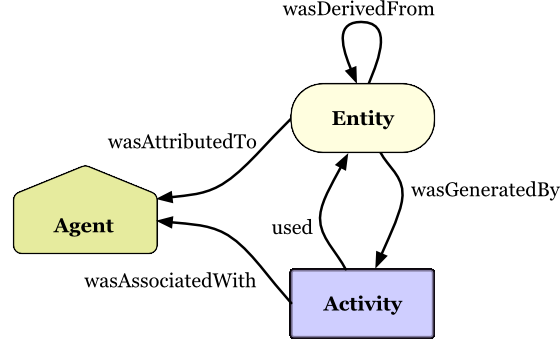
\includegraphics[width=10cm]{fithesis/images/provdm-basics.png}
  \end{center}
  \caption{High level overview of the provenance structures \cite{provdm-basics}.}
  \label{fig:provdm-basics}
\end{figure}

Nodes in a provenance graph represent three types of objects that can be expressed in provenance: Entities, Activities, and Agents. Entities represent snapshots of physical, digital, or other objects central to or associated with the provenance, taken at a concrete point in time. Activities represent actions and processes conducted on or with these entities. Agents are the nodes that perform activities, effectively creating or influencing entities and activities. The edges in a provenance graph represent the relations between these nodes, with examples being 'wasDerivedFrom,' 'wasGeneratedBy,' and 'used.' Both nodes and edges can be referred to as provenance structures.

Each provenance structure has properties the model defines, attributes the user defines, and a unique identifier, which identifies it in the current provenance graph. The identifier is a QualifiedName, which consists of the name of the object it refers to, a namespace that categorizes or contains it, and an optional prefix to represent the namespace more concisely. The PROV-DM supports extensions of its base model, with the users being able to specify types of nodes and edges and add custom attributes; this enhances the flexibility of the PROV-DM.

Moreover, the PROV-DM standard includes a concept known as Bundles, which are used to group sets of provenance structures. Like other provenance structures, a Bundle also has a QualifiedName identifier, which allows it to be represented in a provenance as an Entity, effectively allowing the creation of a provenance of a provenance.
\shorthandon{-}

\subsection{PROV-N}
\shorthandoff{-}
The W3C PROV-N is a component of the W3C PROV suite designed to represent PROV-DM in a human-readable textual format, using files with .provn extension. Each PROV-N file contains a single Document organized into three main sections: namespace declarations, statements, and bundles. A PROV-N document, with declared namespaces and a bundle encapsulating its statements, could look like this snippet:

\begin{center}
\begin{lstlisting}[numbers=left,
    stepnumber=1,
    tabsize=4,
    breaklines=true,
    breakatwhitespace=false,
    xleftmargin=3.5em
    ]
document
  prefix prefix1 <prefix1_URI>

  bundle prefix1:sampleBundle.provn
    prefix prefix1 <prefix1_URI>
    prefix dct <dct_URI>

    entity(prefix1:entity1,[
        prov:type='image',
        dct:format='jpeg',
    ])
  endBundle
endDocument
\end{lstlisting}
\end{center}

Namespace declarations (lines 2, 5, and 6 of the snippet) are a technical means to define qualified names in PROV-N Documents. They shorten the QualifiedName identifiers by specifying a shorthand prefix to a longer namespace URI at the beginning of each Document and Bundle. For instance, a QualifiedName of the Entity from the snippet (line 8) will look as follows:

\begin{verbatim}

    prefix1:prefix1_URI/entity1
    
\end{verbatim}

Statements represent provenance structures. For example, the Entity from the snippet (line 8 of the snippet) is described as "entity(Qual-ifiedName identifier)" with an attribute specifying that the documented object is an image (line 9 of the snippet) and an attribute detailing its characteristics (line 10 of the snippet).

Bundles (line 4 of the snippet) are optional functionality for grouping provenance structures. Provenance structures can be defined outside or inside of a Bundle, but Bundles themselves cannot be folded into each other. Because the QualifiedName of the Bundle from the snippet contains the prefix "prefix1", it must also be declared outside of the Bundle (line 2 of the snippet).
\shorthandon{-}

\section{Provenance chain} \label{s-provchain}
\shorthandoff{-}
The provenance chain is defined in the Common Provenance Model \cite{cpm}, an extension of the PROV-DM for distributed environments. A provenance chain is defined as a sequence of interconnected Bundles, each encapsulating a graph consisting of two parts. The first part is a provenance backbone, a part of the Bundle's graph that serves as a signpost for traversing provenance chains. The backbone contains information about the graph in the given Bundle and establishes connections within and between other Bundles in the chain. Each Bundle in the provenance chain documents an activity that takes inputs and produces outputs, represented by Activity provenance structure with type cpm:mainActivity. Backbone has a pre-defined structure for mapping these inputs to outputs. Therefore, the content of the backbone is not dependent on what specific type of activity is documented.

The second part of a Bundle from a chain is a domain-specific part of the graph. It is a more detailed description of the activity documented in the Bundle; it gives more detailed information compared to what is stored on the backbone. For instance, the domain-specific part can contain information about subactivities of the main Activity or about intermediate products of the whole process. Provenance backbone and domain-specific information are linked in a contiguous graph in a defined way, which is out of the scope of this thesis. This thesis will work only with a part of the provenance backbone relevant to it.

The provenance backbone, as shown in Figure \ref{fig:bundleconnection}, comprises three types of Entities: backwardConnector, currentConnector, and forwardConnector. These Entities are related to each other through the WasDerivedFrom derivation.  

\begin{figure}[htbp]
  \begin{center}
    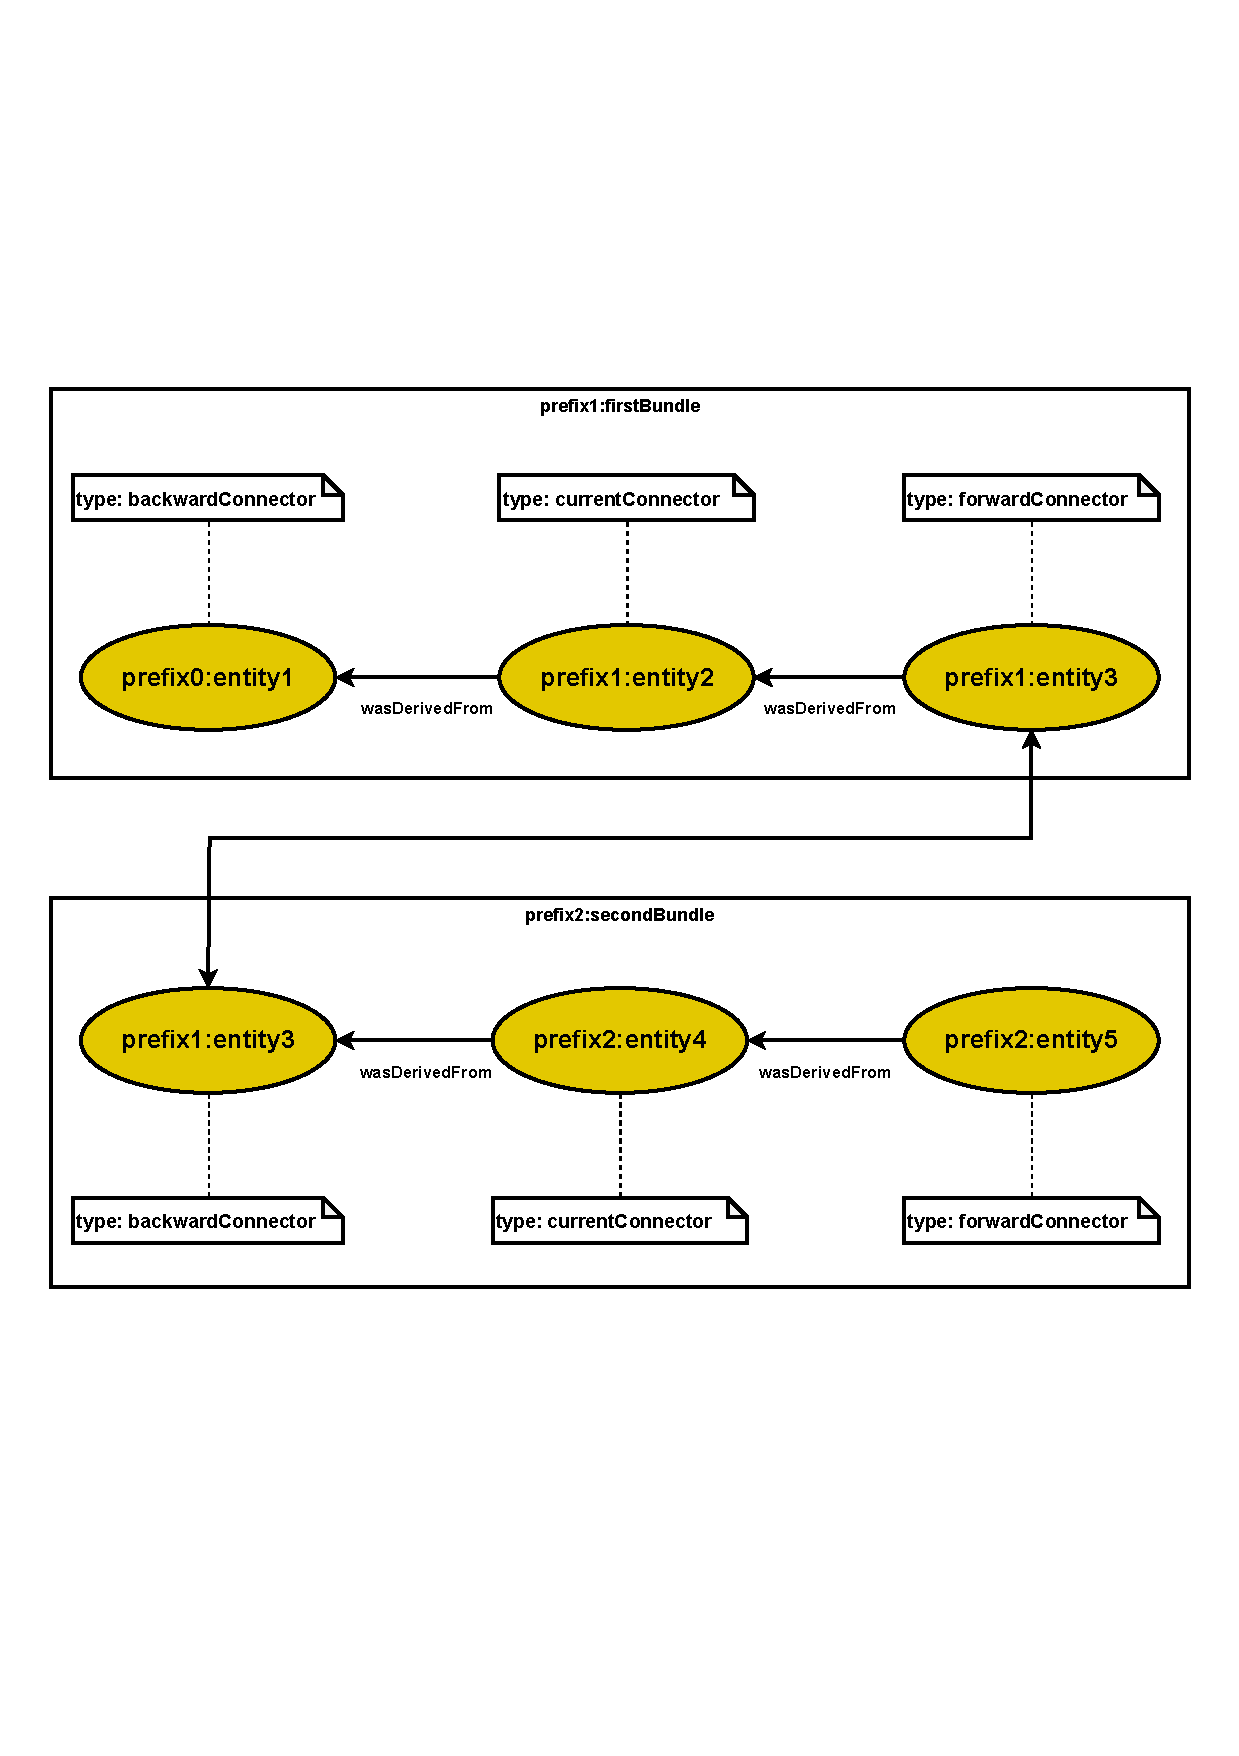
\includegraphics[width=12.5cm]{fithesis/images/backbone.pdf}
  \end{center}
  \caption{Example of a provenance backbone.}
  \label{fig:bundleconnection}
\end{figure}

As mentioned in the Introduction, the provenance chain represents the passing of research objects between various organizations, with each organization documenting only part of its lifecycle.

The backwardConnector represents the documented object at the time it was sent from the sender to the receiver and references the previous Bundle in the chain, where it links to a forwardConnector with the same identifier.

The currentConnector, derived from the backwardConnector, represents the documented object at the time the receiver Bundle received it and references the current Bundle.

The forwardConnector, derived from the currentConnector, represents the documented object at the time it was sent from the current Bundle and references the succeeding Bundle in the chain, where it links to a backwardConnector with the same identifier. If graphs of two succeeding Bundles were to merge, the point of connection of these graphs would be their linked forwardConnector and backwardConnector, both representing the documented object at the same time instant.

The end of the provenance chain can be recognized by connectors missing from a Bundle's backbone. A Bundle missing the backwardConnector and currentConnector represents a starting point in the provenance chain, while a Bundle missing the forwardConnector represents the endpoint \cite{provchain} (Section Distributed Provenance Information \& CPM).

While the example from Figure \ref{fig:bundleconnection} simplifies the structure, in practice, a single bundle can contain multiple connectors of the same type. This multiplicity allows connections to more than one Bundle on either side of the provenance backbone, thereby accommodating complex provenance scenarios.

\shorthandon{-}

\section{Real-world distribution}
The provenance chain is meant to be used in a multi-organizational distributed environment, meaning the bundles of a provenance chain are distributed across multiple companies and that one or more Bundles from the chain represent a company's processing of the provenance's object, effectively documenting its complete lifecycle.

\label{t-aiexample} This thesis works with an example of a provenance chain\footfullcite{provchain-files} consisting of six Bundles, documenting a process of training an AI model to detect tumors on images of prostate tissue. Each Bundle from this provenance chain documents part of the process. The first Bundle documents the collection of a biological sample from a patient. The second Bundle documents the diagnosis and data generation processes. After this, the chain branches out as the third Bundle documents the storage of the sample in a biobank, while another branch continues into the fourth Bundle, documenting the preprocessing of the generated data for AI model training. The fifth Bundle documents the process of the AI model training, and the last Bundle documents the testing of the trained AI model. See the Running example section in \cite{research} for more details.

\section{Additional concepts} \label{concepts}
Additional concepts were developed in order to address issues that tie to the usage of the provenance chain in a distributed environment. One such issue is how to account for versioning of Bundles in the chain. To address it, the meta-provenance is used. Meta-provenance is a Bundle that keeps provenance, like the current version and its hashes, about the Bundles, ensuring that each one links to the correct version of the succeeding Bundles \cite{provchain} (Section Versioning of Distributed Provenance in CPM).

Another concept is the usage of persistent identifier (PID). 
The PID is:

\begin{enumerate}
    \item Globally unique, meaning that it is distinct and distinguishable from all other identifiers across the globe, with no two entities having the same PID.
    \item Persistent, meaning that it ensures that the link to the data or resource remains constant over time, regardless of any changes.
    \item Resolvable, meaning that the PID can be used to locate and access the resource it identifies.
\end{enumerate}

PID management is usually performed by a service where users can register new PIDs by defining what the PID will resolve into. In the case of provenance chains, the PIDs are used to identify connectors and resolve into a quartet of values:

\begin{enumerate}
    \item Entity ID
    \item Connector type of the Entity
    \item ID of a Bundle referenced by the Entity
    \item ID of meta-provenance containing the referenced Bundle
\end{enumerate}

The goal of the PID in provenance chains is to support the validity of the connector identifiers in the long term, i.e., that the links to the other bundles and related information are not deprecated. 


\chapter{Design}
\shorthandoff{-}
This chapter delves into the architecture and logic of the command line tool and its underlying library, both developed as an implementation part of this thesis. The chapter has three main objectives. Firstly, it aims to provide a clear and concise overview of the implementation structure and its components, including their respective roles in its lifecycle. Secondly, it discusses the simulated environment of a real-world distribution and how it works. Finally, it describes the primary logic used to traverse a provenance chain.
\shorthandon{-}

\section{Design overview}
The objective of the implementation is to allow users to perform different operations by entering their associated commands. The main operation is to provide the user with the ability to retrieve precursors or successors of an object documented by an Entity from a provenance chain. For example, in the provenance chain described in Section \ref{t-aiexample}, the user can retrieve precursors of a data set or trained AI model. Another operation is to retrieve the precursors or successors together with the main Activity of their Bundles.

The implementation also contains a secondary library used to generate meta-provenance to keep the provenance of Bundles in the chain with their hashes. This secondary library is used only for the simulation, to be described in \ref{s-simulation}.

\section{Library structure}
\shorthandoff{-}
The implementation is designed as a modular, multi-component library. Central to this structure is a layered architecture, segregating the library operations into four components.

\begin{enumerate}
    \item \textbf{Main UI:}
        The Main UI component is tasked with the initialization of resources for the library and providing a user interface on the command line, where the user can input commands and view the results of the entered queries. The user interface also provides quality-of-life functions, such as command auto-completion, command history, or in-command query history.
    \item \textbf{Configuration:}
        The Configuration component retrieves data from a configuration JSON file and passes it to the library.
    \item \textbf{Tools:}
        The Tools component serves as a toolset for the library, with the first set of tools used to retrieve and deserialize PROV-N documents depending on their storage type. The second set of tools is used to resolve persistent identifiers stored in the relevant navigation table. The third is used for retrieving hash values from the corresponding meta-provenance, and the last is used for hash creation and integrity verification.
    \item \textbf{Main logic:}
        The Main logic component handles the data processing. It traverses the provenance chain and retrieves the user-specified data. It also assures the correctness of the traversed chain by evaluating the integrity of the document using its hash values stored in the corresponding meta-provenance and comparing it to new hash values created using the last set of tools.
\end{enumerate}
\shorthandon{-}

\section{Simulation} \label{s-simulation}
\shorthandoff{-}
This section describes how different aspects of a real-world environment were simulated. The simulation of a distributed environment is performed on a set of six PROV-N files, each containing a single Bundle pre-filled with domain-specific data and a provenance backbone to form a provenance chain as defined in Section \ref{s-provchain}. This provenance chain documents a process from digital pathology described in Section \ref{t-aiexample}. This file set was provided as part of the input by the thesis supervisor. In a real-world environment, every organization would have a public API (e.g., a web service) that could be used to access provenance, and the provenance chain would be traversed using these APIs. This traversal is simulated by a recursive call of a method implementing the Main logic.

When the work on this thesis began, the concept of provenance chains had been developed as a state-of-the-art solution for the representation of distributed provenance. Therefore, how PID resolution and meta-provenance would work still needed to be decided and was not provided by the thesis supervisor as part of the input. Both had to be implemented in this thesis to overcome this issue and simulate their existence in a real-world environment. For meta-provenance, a second library was implemented. This library generates a single meta-provenance containing all Bundles from the chain, along with their versioning information and hashes, which it also generates using the Tools for hash creation. 

To simulate PID resolving, an in-memory navigational table is used. This table consists of all Bundles in the provenance chain. When provided with an identifier of an Entity, it returns the quartet of values as described in Section \ref{concepts}. Access to this table is implemented through a PID-resolving Interface, the inclusion of which allows the implemented library to be extended to other types of PID resolving.
\shorthandon{-}

\section{Provenance chain traversal}
\shorthandoff{-}
This section discusses the traversal of the provenance chain using the provenance backbone and retrieval of precursors or successors of an object represented by an Entity present in the backbone. The inputs for this traversal are identifiers of an Entity and a Bundle containing the Entity. For this example, the traversal moves in a forward direction, retrieving the successors of the Entity. The successors are represented by backwardConnectors because they serve as a representation of the provenance graph's node in the given Bundle, from which it is possible to traverse further within the given Bundle. The structure of the example provenance chain, as shown in Figure \ref{fig:algorithm-Chain}, contains three Bundles. The inputs are \texttt{prefix1:entity1} and \texttt{prefix1:bundle1}.

\begin{figure}[htbp]
  \begin{center}
    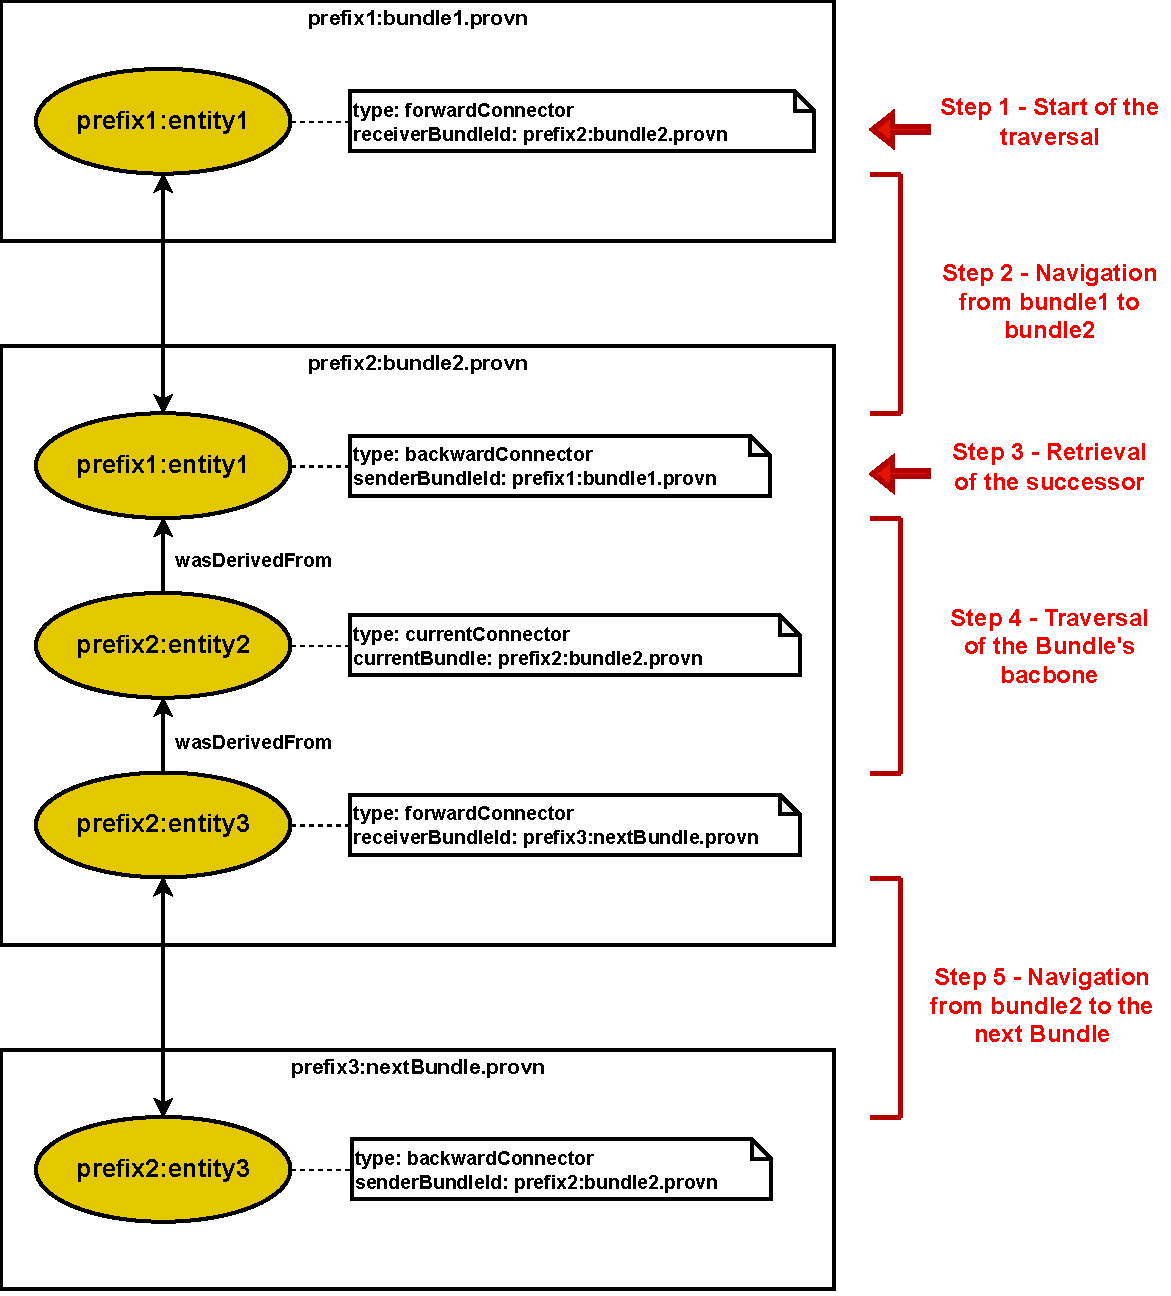
\includegraphics[width=11.5cm]{fithesis/images/algorithm.pdf}
  \end{center}
  \caption{Example of the provenance chain's structure.}
  \label{fig:algorithm-Chain}
\end{figure}
\shorthandon{-}

The steps:
\begin{enumerate}
    \item The traversal begins on the Entity specified in the input.
    \item Considering the traversal is already on the forwardConnector, the first step is to move to the Entity linked to entity1, which is an Entity with the same identifier in the Bundle specified in the receiverBundleId attribute.
    \item Because the traversal is currently on a backwardConnector, the current Entity and Bundle identifiers are added to the list of successors, and the traversal continues.
    \item The next step of the traversal is to move using a graph search algorithm to search for paths of length two, starting from backwardConnector, on edges of type wasDerivedFrom against the direction of the graph's orientation to get again to the forwardConnector.
    \item The traversal moves into the next Bundle using a recursive call to Step 2, and the whole process repeats, retrieving the next successor until no more Entities are derived using the wasDerivedFrom edge or there are no succeeding bundles.
\end{enumerate}

The traversal works analogically for precursors, but the traversal direction follows the graph's orientation, and forwardConnectors are retrieved instead.


\chapter{Implementation}
\shorthandoff{-}
This chapter aims to establish a connection between the theoretical framework discussed in the Design chapter and the practical implementation of the tool. Firstly, it provides a listing of used libraries and a description of their usage in the implementation. After that, it offers an in-depth look at the code structure. It follows with a description of the implementation's runtime and finishes with a section about problems that arose during the implementation.

\section{Used technologies}
The following part delves into the libraries and tools used in the implementation and the reasoning behind the usage of each. Each library and tool has been chosen and integrated into the implementation to address specific functional requirements and enhance the application's usability, efficiency, and interoperability.

\subsection{ProvToolBox}
The ProvToolBox \cite{provtoolbox} is a common library for handling provenance according to PROV DM; classes and interfaces of the library implement various aspects of the data model, such as Entites, Activities, Agents, Relations, provenance Documents, or Bundles. It consists of multiple components, each focusing on some aspect of provenance management in the code. Two of these components, the prov-model and prov-interop-light, are used in this implementation. The prov-model is used across the whole implementation to create and manipulate provenance documents. The prov-interop-light facilitates the conversion of the in-memory data model into various formats, ensuring that the application can communicate effectively with other provenance-aware systems and tools.
\subsection{Jackson Databind}
Jackson Databind \cite{jackson} is a library for handling JSON data formats. It parses the JSON configuration file and creates Java objects from it.
\subsection{GitLab4J API}
The GitLab4J API \cite{gitapi} is a library to facilitate interaction with GitLab's APIs. It automates file retrieval, allowing the library to support git-based provenance storage.
\subsection{JLine Bundle}
JLine Bundle \cite{jline} is a library used to enhance the user interface of the implementation. It provides capabilities such as command-line completion and history, significantly improving the user experience by making the interface more intuitive and responsive.
\subsection{Jansi}
Jansi \cite{jansi} is a library used to improve formatting options of the console output. It renders text in different colors and styles, making the console output about the integrity of Bundles more readable and user-friendly.
\subsection{Apache Maven Shade Plugin}
The Maven Shade Plugin \cite{maven-shade} creates an uber-jar, a standalone executable jar file containing all the necessary dependencies. This approach simplifies deployment and distribution, ensuring the library is self-contained and can be run in diverse environments without additional dependency management.
\section*{}


\section{Project structure}
The tool was implemented as a Maven project using the IntelliJ IDEA from JetBrains. This section serves as an overview of the implementation's project structure, providing insight into the classes and their methods in each of the project's packages.

\newpage
\subsection{Configuration}
\dirtree{%
.1 provenancechain.
.2 config.
.3 ConfigLoader.java.
.3 Configuration.java.
.2 ....
}
\vskip 0.35cm

The config package comprises two classes for loading configuration data from a JSON file using the Jackson Databind library. The \texttt{Configuration} class specifies the data type or object the deserialized data will be cast into, depending on their name and the properties of the JSON file. The \texttt{ConfigLoader} class contains the main logic for JSON file deserialization.

\subsection{Tools}
\dirtree{%
.1 provenancechain.
.2 ....
.2 tools.
.3 loading.
.4 ....
.4 IFileLoader.java.
.4 LoaderResolver.java.
.4 SupportedExtensions.java.
.3 metadata.
.4 IPidResolver.java.
.3 retrieving.
.4 IMetaHashRetriever.java.
.3 security.
.4 HashDocument.java.
.4 IntegrityVerifier.java.
}
\vskip 0.35cm

The tools package consists of four sub-packages, each with a set of specific tools. 

The loading sub-package consists of tools used for file deserialization. The \texttt{IFileLoader} interface is used to implement file deserialization depending on the type of storage, with current implementations being for GitLab and the local file system. The \texttt{LoaderResolver} class is used to choose the correct implementation of the \texttt{IFileLoader}, and the SupportedExtensions enum is used to avoid unsupported file types. 

The metadata sub-package consists of an \texttt{IPidResolver} interface used to implement resolving and access to the navigational table for different types of PIDs. 

The retrieving sub-package consists of an \texttt{IMetaHashRetriever} interface used to implement the retrieval of hash values from the meta-provenance. 

Lastly, the security sub-package consists of tools used for operations with hashes. The \texttt{HashDocument} class contains methods to create hashes for Documents, with SHA-256 and MD5 currently being the only techniques supported. The \texttt{IntegrityVerifier} class contains a static method to compare existing hashes from meta-provenance with newly created ones.

\subsection{Simulation}
\dirtree{%
.1 provenancechain.
.2 ....
.2 simulation.
.3 ....
.3 Initializer.java.
.3 SimulationFiles.java.
.2 ....
}
\vskip 0.35cm

The simulation package is used to hold implementations of interfaces from the tools package and other classes used for the simulation in this thesis. The \texttt{SimulationFiles} class is similar in structure to the \texttt{IFileLoader} implementations in the loading sub-package. However, it is used to load and prepare copies of the provided files saved in the project's resources to be used for simulation purposes. The \texttt{Initializer} class implements the building process of the simulation. It uses the \texttt{SimulationFiles} class to retrieve the provided files that represent the provenance chain and uses them to generate a meta-provenance and to create a navigational table. It also provides a static method to access this navigational table.

\newpage
\subsection{Main logic}
\dirtree{%
.1 provenancechain.
.2 ....
.2 logic.
.3 data.
.4 ProvenanceNode.java.
.3 Crawler.java.
.2 ....
.2 MainRuntime.java.
}
\vskip 0.35cm

The logic package and the \texttt{MainRuntime} class serve as the main logic of the implementation. The \texttt{MainRuntime} initializes the required resources for the implementation to work and provides a user-friendly command line interface for the user to enter commands. The supported commands are:

\begin{enumerate}
    \item "exit" to exit the program
    \item "precursors"/"successors" to print the precursors or successors of an object represented as an Entity on the backbone.
    \item "precursors-activity"/"successors-activity" to print the precursors or successors of an object represented as an Entity on the backbone with the inclusion of the main Activity for each Bundle in the chain.
    \item "resolve" to resolve a given PID by retrieving data from the navigational table for a specified object represented as an Entity on the backbone.
    \item "list" to print out the whole navigational table
    \item "help" to list all supported commands.
\end{enumerate}

The \texttt{Crawler} class contains the methods for traversing the provenance chain and retrieving the precursors or successors. The \texttt{Provenan}-\texttt{ceNode} class represents a node in the provenance graph and is used to store and represent the retrieved precursors or successors.

\section{Execution walkthrough}
This section is intended to provide a concise walkthrough of the implementation's execution. The purpose is to offer insight into how different classes and components interact to produce the desired results for the user. By reading this walkthrough, readers will understand the underlying mechanisms of the operations performed during the execution. 

The execution begins by calling the method main in the class \texttt{Main}. The initialization from the \texttt{MainRuntime} class is performed, followed by the calling of its run method.

\subsection{Initialization}
The initialization performed by the \texttt{MainRuntime} class consists of three parts. The first part is the retrieval of data from the configuration JSON file. The second part is the initialization of the simulated environment. This part loads the provided provenance files, which are saved in the project resources. These files are then used to generate a meta-provenance using the sublibrary described in Section \ref{s-simulation}. In addition to generating the meta-provenance, this part also generates a simulated navigational table using the same files. The last part is the initialization of the remaining resources for the implementation to work.

\subsection{Runtime}
After calling the run method from the \texttt{MainRuntime} class, a command line interface is provided for the user to enter commands. For this walkthrough, the request is to retrieve the precursors of an Entity by using the 'precursors' command. The mentioned precursors are represented by the QualifiedName identifiers of forwardConnector Entities of the preceding Bundles. Refer to \ref{fig:runtime} for a better picture of the runtime.

\begin{figure}[htbp]
  \begin{center}
    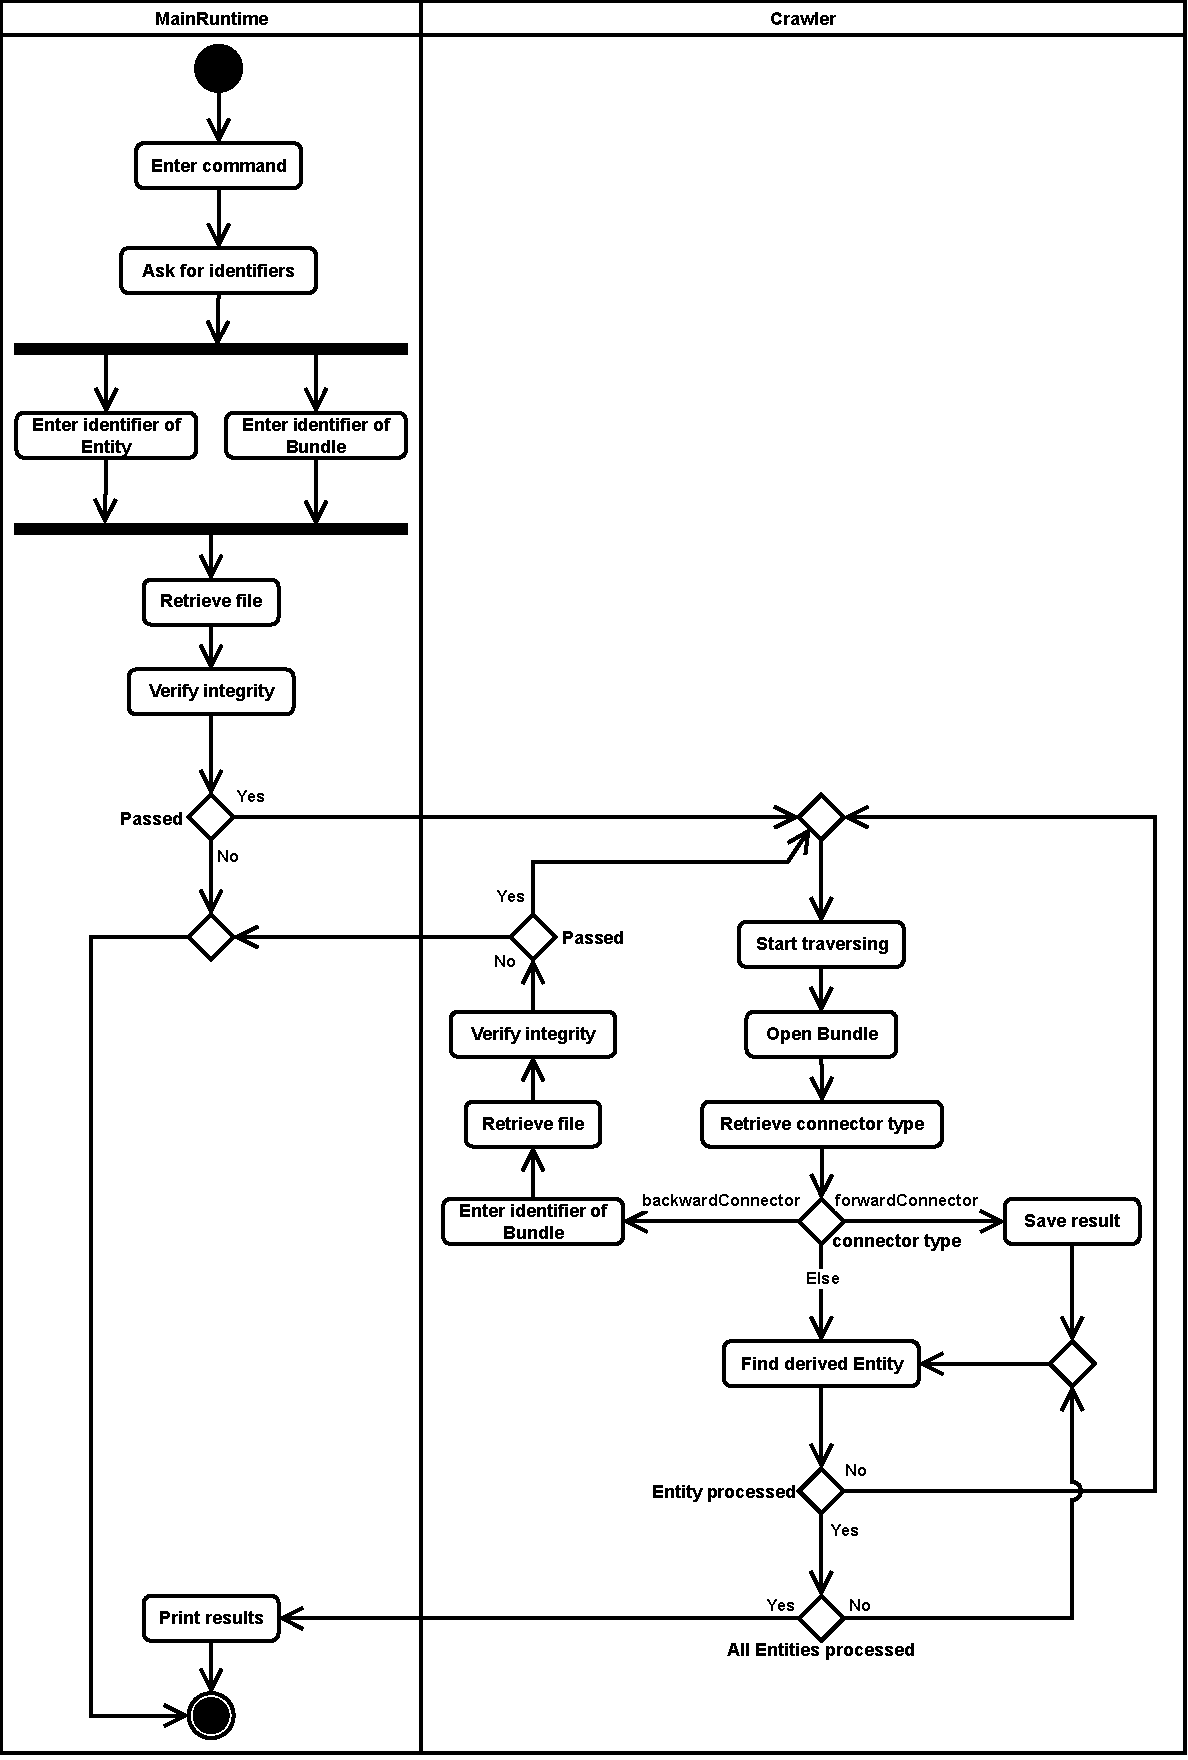
\includegraphics[width=12cm]{fithesis/images/runtime.pdf}
  \end{center}
  \caption{High level Activity diagram of the 'precursors' command.}
  \label{fig:runtime}
\end{figure}
 
Afterward, the user is prompted to enter a connector's ID and URI and the ID and URI of a Bundle whose backbone contains the entered connector. Next, the correct implementation of the IFileLoader interface is chosen depending on what type of storage the Bundle's URI is pointing to, and the PROV-N file, with a name matching the Bundle's ID, is returned deserialized into a Document object. After that, the integrity of the Document is verified by calling the static checkSum method of the \texttt{IntegrityVerifier} class. This method compares this Document's newly created hash with its hash in the meta-provenance. With a successful integrity verification, the runtime enters the Crawler's method getPrecursors.

Upon entering, the proper navigational table resolver is chosen using the getPidResolver method. As part of the simulation in this thesis, the getPidResolver method is set to always return the simulated resolver. Next, the Bundle inside of the Document is retrieved and the type of the current connector is found. 

If the type is a forwardConnector, the connector's identifier and its Bundle's identifier are added to the list of precursors. The connector's identifier is also added to the list of processed nodes, and the method continues. 

If the type is a backwardConnector, it means the method reached the end of the current Bundle's backbone, and the same process as in the MainRuntime section repeats. The method uses the connector's entry in the navigational table to retrieve the identifier of the Bundle to which the connector is pointing. The following Document is retrieved using this information, and its integrity is again verified. The connector's identifier is added to the list of processed nodes, and the getPrecursors method is called with the same connector's identifier and the newly loaded Document. 

If the type is neither, the method will search through the WasDerivedFrom statements in the current Bundle to find which connector is following in the traversal. It will then add this connector's identifier to the list of processed nodes and call the getPrecursors method with the current Document and the newly found connector's identifier. 

After the runtime processes all Bundles in the chain and there are no more unprocessed connectors to enter, the traversal ends. The retrieved precursors are then printed on the command line, along with confirmation of the verified integrity of each Bundle. For an example, see Figure \ref{fig:precursor-run}. It should be mentioned that the implementation expects the chain to be correct, as the thesis supervisor stated that it should not focus on verification of whether the chain is cycled.

\begin{figure}[htbp]
  \begin{center}
    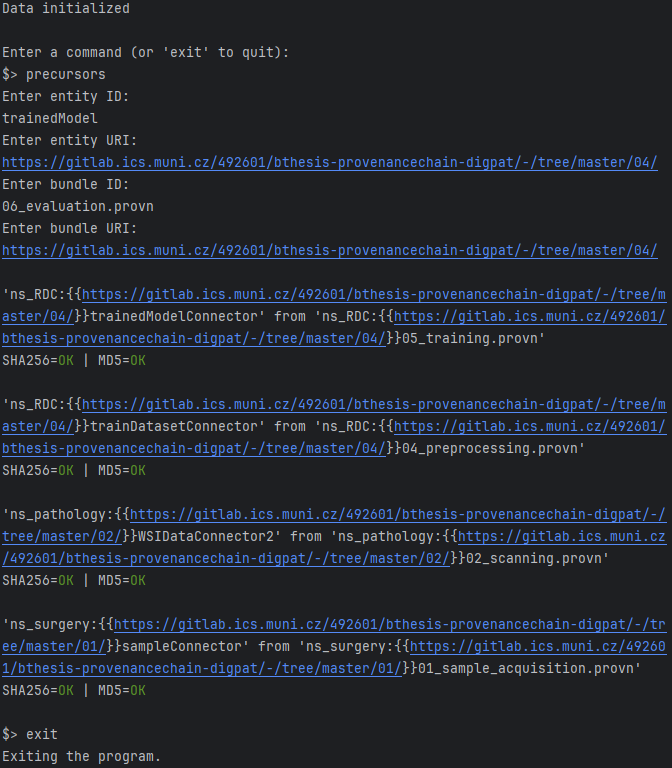
\includegraphics[width=12.5cm]{fithesis/images/precursor-run-slim.png}
  \end{center}
  \caption{Example of execution with the 'precursors' command.}
  \label{fig:precursor-run}
\end{figure}

\section{Problems during implementation}
Four problems were encountered during the implementation due to incompatibilities between the used Java library and the Python library used by the thesis supervisor to generate the input files. The first three problems arose from the simulation files, provided by the thesis supervisor, being generated using a Python library, which produced files with some notation differences. The first is that the Python library supports attributes with multiple values using parentheses, while the Java library needs each attribute to have only one value.

\begin{verbatim}

    Python: 
        dct:hasPart=('prefix:local1','prefix:local2')
    Java:
        dct:hasPart='prefix:local1', 
        dct:hasPart='prefix:local2' 
        
\end{verbatim}

The second problem came from the Python library supporting the creation of Entities with space in names, which is seen as a syntax error by the Java library.

\begin{verbatim}

    Python:
        entity(prefix:local 1, [prov:type=...
    Java:
        entity(prefix:local_1, [prov:type=... 
        
\end{verbatim}

The third problem was caused because the Python library generates attributes with values encompassed by double quotes. The Java library differentiates between single and double quotes. The single quotes are resolved as the QualifiedName specified inside of them.

\begin{verbatim}

    cpm:receiverBundleId='prefix:local.provn'
    
    Resolved:
        'prefix:{{uri}}local.provn'
        
\end{verbatim}

While the double quotes are regarded as a LangString

\begin{verbatim}

    cpm:receiverServiceUri="prefix:local.provn"
    
    Resolved:
        LangString@xxx[value=prefix:local.provn,lang=<null>]
        
\end{verbatim}

These findings about the libraries' differences were then reported to the thesis supervisor and were corrected in the provided files to use the Java-compatible notation.

The last problem came from the fact that the ProvToolBox library, at the time of thesis implementation, was left on version 0.9.3, with the last update being over three years ago, which caused some of the library's features not to work correctly or at all. One such feature was a method getEntity used to return an Entity with specified QualifiedName from a Bundle. The library's GitHub page had an open issue from 2019 about a similar method used to return an Agent instead of an Entity. To possibly remind the authors about the issue, a reply was posted as the specifications in the issue also applied to the getEntity method. The absence of this method in the implementation was compensated by looping over the Entities inside of a Bundle and finding the Entity with the same identifier. As of the late summer of 2023, the development seems to have returned, with new updates being released, and the mentioned issue being resolved and closed.
\shorthandon{-}


\chapter{Manual}
\shorthandoff{-}
This chapter describes the set-up of the implemented tool on a Windows system. It describes the set-up process for the submitted archive and, in case the archive does not work or is no longer accessible, for the git repository containing the implementation.

\section{Archive}
The submitted archive contains a fully initialized maven project, a compiled jar, and an installation file, each provided for different scenarios:

\begin{enumerate}
    \item If neither Maven nor Java is appropriately configured, the user can install the implementation using the ProvenanceChain-1.0.m-si file. This will install the implemented tool together with a bundled Java Runtime Environment. The tool will be installed in the Program Files folder under ProvenanceChain and can be run by executing the ProvenanceChain.exe file. As part of the simulation, executing the installed tool will create a meta\_provenance.p-rovn file in the current user's Documents folder. This file can be deleted after the tool's execution, and the tool itself can be uninstalled as any other application in the Windows settings.
    \item If Java is configured on the target system, the tool can be run by executing the run.bat file inside the bthesis-provenancechain folder.
    \item In the scenario where neither the installer nor the jar file work, the tool can be built and executed using the provided maven project, that is, the bthesis-provenancechain folder. This approach requires a configured Maven and Java as well as an IDE.
\end{enumerate}

To try the tool, use the command \textbf{\texttt{'precursors'}} and provide this set of inputs: 
\begin{verbatim}

Entity ID: trainedModel

Entity URI: https://gitlab.ics.muni.cz/492601/bthesis
-provenancechain-digpat/-/tree/master/04/

Bundle ID: 06_evaluation.provn

Bundle URI: https://gitlab.ics.muni.cz/492601/bthesis
-provenancechain-digpat/-/tree/master/04/

\end{verbatim}

The following execution should produce the same results, as shown in Figure \ref{fig:precursor-run}

\section{Git}
In case the submitted archive fails or is no longer available, the implementation can be retrieved from a Git repository following this manual.

\subsection{Set-up}
To utilize the implemented tool, it is necessary to have Maven and Java properly configured. To simplify the process for users, the implementation is currently spread across multiple Git repositories, including two on FI \cite{provchain-fi} and ICS \cite{provchain-ics} GitLab sites and one on the author's personal GitHub page \cite{provchain-github}. To obtain the tool, clone the repository or use the download button to retrieve the entire repository bundled in a zip or another archive file.

\subsection{Simulating the environment}
The initiation of simulation files is the first step in simulating the environment. It requires the retrieval of provenance files necessary for the simulated environment to function effectively. To achieve this, a submodule in the repository must be initialized. Start by opening the cloned repository in a command line and navigating to the submodule's folder using the following command.

\begin{verbatim}
$ cd. \src\main\resources\bthesis-provenancechain-digpat  
\end{verbatim}

Once the submodule is reached, the command 

\begin{verbatim}
$ git submodule foreach git fetch –tags
\end{verbatim}

should be executed. After it finishes, there should be no output. Finally, the command

\begin{verbatim}
$ git submodule update --init --recursive  
\end{verbatim}

should be run to conclude the process. This will ensure that the bthesis-provenancechain-digpat submodule contains the required .provn files.

\subsection{Building}
The jar file is packaged using the Maven Shade plugin, which is the preferred method. To create the jar file, navigate to the cloned repository using the console and run the \textbf{\texttt{mvn clean package}} command. After creating the jar file, it can be launched by executing the command \textbf{\texttt{java -jar }\path{.\target\BThesis-ProvenanceChain-VERSION-shaded.jar}}.

In the event that the intended environment does not have a JRE, the \textbf{\texttt{jpackage}} command line tool provided by Java can be used to create a platform-specific installer.

\section{Omitting the simulated environment}
The implementation employs several classes and files that provide the necessary objects to simulate the real-world environment. To enhance clarity, these classes have been transferred to packages labeled 'bthesis.provenancechain.simulation' and 'bthesis.metageneration'. At the same time, the required files reside in the previously mentioned submodule 'src.main.resources.bthesis-provenancechain-digpat'. However, these components can be omitted if the required classes are adequately substituted.
\shorthandon{-}


\chapter*{Conclusion}
\markright{\textsc{Conclusion}}
\addcontentsline{toc}{chapter}{Conclusion}
\shorthandoff{-}
This thesis describes a command line tool and its underlying library for traversing provenance chains developed as the implementation part of the thesis. The thesis begins with the Provenance chapter, delving into the theoretical framework of provenance. It explains the PROV-DM data model and the PROV-N notation developed by the World Wide Web Consortium (W3C). The chapter also introduces the concept of a provenance chain and its real-world applications, especially in medical research, and discusses additional concepts like meta-provenance and persistent identification. The Design chapter focuses on the architecture and logic of the implemented command line tool. It discusses the modular design of the system, its components, and their functionalities. The chapter further describes the simulation of a real-world environment and the primary logic for traversing a provenance chain. The Implementation chapter offers an in-depth look at the code structure and the libraries and tools used in the project. This chapter also provides an execution walkthrough and addresses the challenges encountered during the implementation process. The Manual chapter serves as a guide for setting up and using the implemented tool. It provides detailed instructions on simulating the environment, building the tool, and executing various functions. It also discusses how to omit the simulated environment for different application contexts.

The main output of this thesis is a successful implementation of a command line tool and its underlying library for provenance chain traversing, running on a set of PROV-N files, effectively simulating a real-world environment. The modular design of the system and the insights gained from the challenges encountered offer a solid foundation for future enhancements and adaptations. Additionally, the implemented library was used for validation of the results of the scientific paper, the preprint of which is available at \cite{preprint}. The validation of the results was added to the paper in the first major revision and is not part of the cited preprint.

For future research, several directions can be explored. The scalability of the provenance chain traversal system in more complex and distributed environments by transitioning from the current recursive method call approach to a service-oriented architecture. In this model, individual services would be deployed, each responsible for handling a segment of the provenance chain. These services can manage requests and return responses either synchronously or asynchronously.

Another aspect to explore is the modification of the system's core logic. Currently, the system utilizes a recursive call method to traverse the provenance backbone. A potential improvement could involve replacing this recursive call with an iterative approach. This change would optimize the system's performance by reducing the stack overhead associated with recursive calls. Additionally, the integration of advanced security features like authorization models or access control to ensure the integrity and confidentiality of provenance data is an area that could yield significant benefits. Lastly, exploring the application of this system in different domains, such as healthcare or finance, could reveal new use cases for provenance chain management.
\shorthandon{-}

\printbibliography[heading=bibintoc]

\end{document}
